\section{PrePostTest}
\usetikzlibrary{quotes,angles,calc}
\newcommand{\tikzAngleOfLine}{\tikz@AngleOfLine}                               
  \def\tikz@AngleOfLine(#1)(#2)#3{%                                            
  \pgfmathanglebetweenpoints{%                                                 
    \pgfpointanchor{#1}{center}}{%                                             
    \pgfpointanchor{#2}{center}}                                               
  \pgfmathsetmacro{#3}{\pgfmathresult}%                                        
  }  
																																						
\newcommand{\degrees}{
\square \hspace{0.5cm} 30^\circ \newline
\square \hspace{0.5cm} 45^\circ \newline
\square \hspace{0.5cm} 60^\circ \newline
\square \hspace{0.5cm} 90^\circ \newline
\square \hspace{0.5cm} 120^\circ \newline
\square \hspace{0.5cm} 150^\circ \newline
\square \hspace{0.5cm} 180^\circ 
}

\newcommand{\anglePaint}[2]{
	\begin{tikzpicture}[scale=3,line width=1pt, baseline=(current bounding box.north)]                                    
		\coordinate (A) at (0,0);                                                    
		\coordinate (B) at ($(A)+(#1:1)$);                                                    
		\coordinate (C) at ($(A)+(#2:1)$);                                                
		\draw (A) -- (B);                                            
		\draw (A) -- (C);                                            
		\tikzMarkAngle{(A)}{(B)}{(C)}   
	\end{tikzpicture}  
}

\newcommand{\tikzMarkAngle}[3]{                                                
\tikzAngleOfLine#1#2{\AngleStart}                                              
\tikzAngleOfLine#1#3{\AngleEnd}                                                
\draw #1+(\AngleStart:0.15cm) arc (\AngleStart:\AngleEnd:0.15cm);              
}   



%Start of test
\begin{questions}
\question What is an angle?
\question Draw an angle
\question Draw a bigger angle


\question Which angle is bigger in each pair?

\begin{tikzpicture}[thick, scale= 2]
	\draw (0,0) -- (0:1);
	\draw (0,0) -- (80:1);
	\begin{scope}[shift={(2,0)}]
		\draw (0,0) -- (60:2);
		\draw (0,0) -- (20:2);
  \end{scope}
\end{tikzpicture}

\bigskip

\begin{tikzpicture}[thick, scale= 2]
	\draw (0,0) -- (45:1);
	\draw (0,0) -- (-45:1);
	\begin{scope}[shift={(2,0)}]
		\draw (0,0) -- (-45:1);
		\draw (0,0) -- (-135:1);
  \end{scope}
\end{tikzpicture}

\bigskip

\begin{tikzpicture}[thick, scale= 2]
	\draw (0,0) -- (60:1);
	\draw (0,0) -- (80:1);
	\begin{scope}[shift={(2,0)}]
		\draw (0,0) -- (40:1);
		\draw (0,0) -- (10:1);
  \end{scope}
\end{tikzpicture}

\bigskip

\question Find the missing measures of the angles                                                            

%Triangle
\begin{tikzpicture}[scale=4,line width=1pt]                                    
  \coordinate (A) at (0,0);                                                    
  \coordinate (B) at ($(A)+(90:1)$);                                                    
  \coordinate (C) at ($(B)+(-30:2)$);                                                
  \draw (A) -- (B) -- (C) -- cycle;                                            
	
  \tikzMarkAngle{(C)}{(B)}{(A)}   
	\node at ($(C)+(170:0.40)$) {?=\underline{\hspace{1cm}}};
	
	\tikzMarkAngle{(A)}{(B)}{(C)}
	\node at ($(A)+(45:0.25)$) {$90^\circ$};
	
	\tikzMarkAngle{(B)}{(A)}{(C)}           
	\node at ($(B)+(-60:0.25)$) {$60^\circ$};
\end{tikzpicture}  

\bigskip

%Quadliteral
\begin{tikzpicture}[scale=4,line width=1pt]                                    
  \coordinate (A) at (0,0);                                                    
  \coordinate (B) at ($(A)+(80:1)$);                                                    
  \coordinate (D) at ($(A)+(0:3)$);                                                
	\coordinate (C) at ($(D)+(100:1.5)$);
  \draw (A) -- (B) -- (C) -- (D) -- cycle;                                            
	
  \tikzMarkAngle{(A)}{(B)}{(D)}   
	\node at ($(A)+(45:0.25)$) {$80^\circ$};
	
	\tikzMarkAngle{(C)}{(B)}{(D)}           
	\node at ($(C)+(-135:0.25)$) {$90^\circ$};
	
	\tikzMarkAngle{(D)}{(A)}{(C)}          
	\node at ($(D)+(135:0.25)$) {$80^\circ$};
	
	\draw[shift={(B)}] (-100:0.15cm) arc (-100:10:0.15cm);
	\node at ($(B)+(-35:0.40)$) {?=\underline{\hspace{1cm}}};
\end{tikzpicture}  

\bigskip

%Parallelogram
\begin{tikzpicture}[scale=4,line width=1pt]                                    
  \coordinate (A) at (0,0);                                                    
  \coordinate (B) at (2,0);                                                    
  \coordinate (C) at ($(B)+(150:1)$);                                                
	\coordinate (D) at ($(A)+(150:1)$);                                                
  \draw (A) -- (B) -- (C) -- (D) -- cycle;                                            
	
  \tikzMarkAngle{(A)}{(B)}{(D)}   
	\node at ($(A)+(75:0.25)$) {?=\underline{\hspace{1cm}}};
	
	\tikzMarkAngle{(B)}{(A)}{(C)}
	\node at ($(B)+(170:0.40)$) {?=\underline{\hspace{1cm}}};
	
	\tikzMarkAngle{(C)}{(B)}{(D)}    
	\node at ($(C)+(255:0.25)$) {?=\underline{\hspace{1cm}}};
				
	\draw[shift={(D)}] (-30:0.15cm) arc (-30:0:0.15cm);      
	\node at ($(D)+(-13:0.3)$) {$30^\circ$};
\end{tikzpicture} 

\bigskip

%Parallel lines
\begin{tikzpicture}[scale=2, line width=1pt]
  \coordinate (A) at (-2,0);                                                    
  \coordinate (B) at (3,0);                                                    
  \coordinate (C) at ($(60:2) + (-3,0)$);                                                
	\coordinate (D) at ($(60:2) + (2,0)$);                                                
	\coordinate (E) at (60:-1);                                                
	\coordinate (F) at (60:3);                                                
	
	\draw (A) -- (B);
	\draw (C) -- (D);
	\draw (E) -- (F);
	
	\draw (180:0.25cm) arc (180:0:0.25cm); 
	\draw[shift={(60:2)}] (0:0.25cm) arc (0:-180:0.25cm); 
	
	\node at ($(60:2)+(-160:0.7)$) {?=\underline{\hspace{1cm}}};
	\node at ($(60:2)+(-50:0.6)$) {?=\underline{\hspace{1cm}}};
	\node at ($(30:0.5)$) {$60^\circ$};
	\node at ($(130:0.6)$) {?=\underline{\hspace{1cm}}};
\end{tikzpicture}

\question Estimate the angles

\begin{table}[H]
    \begin{tabular}{ p{4cm} r }
    \degrees & \anglePaint{-70}{-100} \\
		\\
		\degrees & \anglePaint{90}{180} \\
		\\
		\degrees & \anglePaint{30}{90} \\
		\\
		\degrees & \anglePaint{60}{20} \\
    \end{tabular}
\end{table}

\question Circle all the angles(if a figure has more than one angle, circle each one).

\begin{figure}[H]
\centering
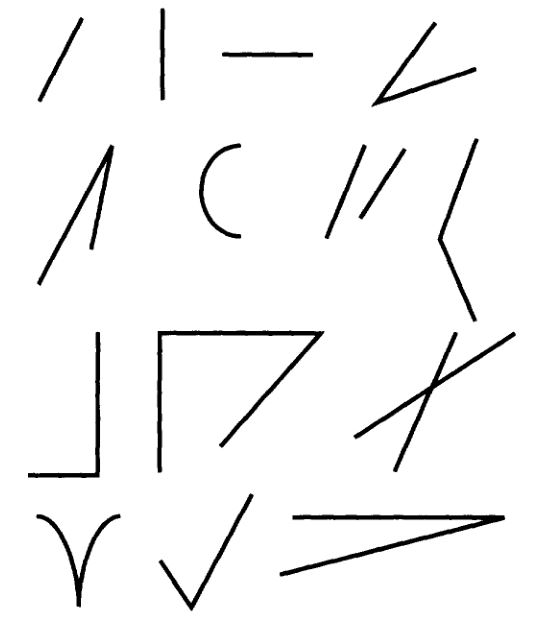
\includegraphics[width=90mm]{anglesTest.jpg}
\end{figure}

\question How many degrees and in which direction (right or left) should you turn the spinner arrow to aim it directly at the center of the target?

\begin{figure}[H]
\centering
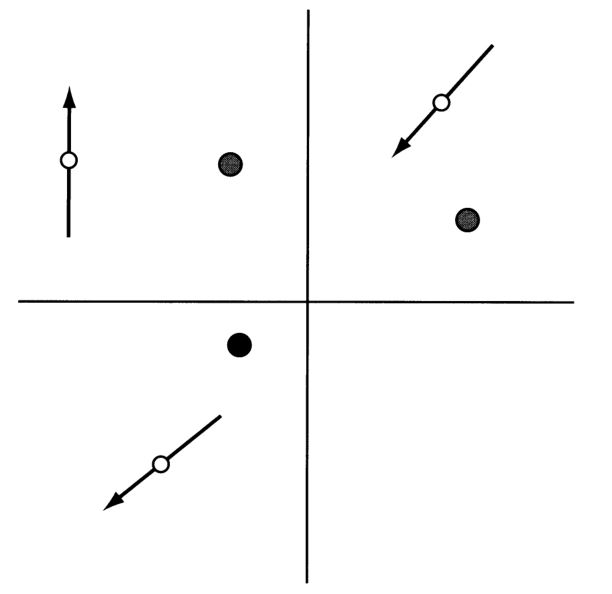
\includegraphics[width=90mm]{turnTest.jpg}
\end{figure}

\question A robot turns 90 degrees every time it turns. How many turns must the robot make before it is facing in the same direction as it was when it started?

\question Another robot turns 30 degrees every time it turns. How many turns must this robot make before it is facing in the same direction as it was when it started?

\question The figure below has 6 angles. All the angles are equally big. How big is each angle?

\begin{tikzpicture}[scale=2, line width=1pt]
  \coordinate (A) at (0,0);                                                    
  \coordinate (B) at ($(A) + (0:1)$);                                                    
  \coordinate (C) at ($(B) + (60:1)$);                                                
	\coordinate (D) at ($(C) + (120:1)$);                                                
	\coordinate (E) at ($(D) + (180:1)$);                                                
	\coordinate (F) at ($(E) + (-120:1)$);                                                
	
	\draw (A) -- (B) -- (C) -- (D) -- (E) -- (F) -- cycle;
	
	\tikzMarkAngle{(A)}{(B)}{(F)}
	\tikzMarkAngle{(B)}{(A)}{(C)}
	\tikzMarkAngle{(C)}{(B)}{(D)}
	\tikzMarkAngle{(D)}{(E)}{(C)}
	\draw[shift={(E)}] (-0:0.15cm) arc (-0:-120:0.15cm);
	\draw[shift={(F)}] (60:0.15cm) arc (60:-60:0.15cm);
\end{tikzpicture}
	
\question Do you think you can learn about angles and degrees using robotics?

\end{questions}
